\documentclass[11pt,a4paper]{article}

\usepackage[margin=1in]{geometry}
\usepackage{mathptmx}
\usepackage{amsmath}
\usepackage{amssymb}
\usepackage{amsthm}
\usepackage{braket}
\usepackage{tikz}
\usetikzlibrary{shapes.geometric}
\usepackage{quantikz}
\usepackage{enumitem}
\usepackage{hyperref}
\usepackage{xcolor}

\definecolor{circuitblue}{RGB}{40,80,160}

\hypersetup{
    colorlinks=true,
    linkcolor=circuitblue,
    urlcolor=circuitblue,
    citecolor=circuitblue
}

\theoremstyle{definition}
\newtheorem{definition}{Definition}[section]
\newtheorem{example}{Example}[section]
\newtheorem{theorem}{Theorem}[section]

\theoremstyle{remark}
\newtheorem*{intuition}{Intuition}
\newtheorem*{keypoint}{Key Point}

\pagestyle{plain}

\setlength{\parindent}{0pt}
\setlength{\parskip}{6pt}

\begin{document}

\begin{center}
    {\LARGE \textbf{Quantum Kernels and SVMs}}\\[8pt]
    {\large QML}\\[12pt]
    \hrule
\end{center}

\vspace{12pt}
\tableofcontents
\newpage

%% ========================================================
\section{Overview}
%% ========================================================

last lecture we built the practical pipeline for quantum kernels --- from qiskit implementation to benchmarking on toy datasets. now we go deeper into the SVM side of things and tackle the real challenges: training on actual datasets, cross-validation, hyperparameter tuning, and understanding when quantum kernels r worth the effort.

this lecture covers:
\begin{itemize}[leftmargin=*]
    \item QSVC in detail --- the complete classifier pipeline with all the math
    \item QSVR --- regression with quantum kernels
    \item pegasos QSVC --- a faster online training algorithm
    \item kernel matrix analysis --- eigenvalue spectra and wt they tell u
    \item training on real datasets: iris, wine, breast cancer
    \item cross-validation with expensive quantum kernels
    \item hyperparameter tuning strategies
    \item computational cost analysis
    \item comparison with classical kernels --- when quantum wins and when it doesnt
    \item limitations and when NOT to use quantum kernels
\end{itemize}

tbh this is the ``reality check'' lecture. we r going to be honest about wt works, wt doesnt, and wt the actual computational costs r.

%% ========================================================
\section{QSVC: Quantum Support Vector Classifier}
%% ========================================================

lets start with the full mathematical treatment of QSVC. this is just a classical SVM with a quantum kernel, but the details matter.

\subsection{The Optimization Problem}

given training data $\{(\mathbf{x}_i, y_i)\}_{i=1}^M$ with $y_i \in \{-1, +1\}$ and a quantum kernel $\kappa(\mathbf{x}, \mathbf{x}') = |\braket{\phi(\mathbf{x})|\phi(\mathbf{x}')}|^2$, the SVM primal problem is:

\begin{definition}[QSVC Primal Problem]
\[
\min_{\mathbf{w}, b, \boldsymbol{\xi}} \frac{1}{2}\|\mathbf{w}\|^2 + C \sum_{i=1}^M \xi_i
\]
subject to:
\begin{align}
y_i(\mathbf{w} \cdot \phi(\mathbf{x}_i) + b) &\geq 1 - \xi_i, \quad i = 1, \ldots, M \\
\xi_i &\geq 0, \quad i = 1, \ldots, M
\end{align}
where $\phi(\mathbf{x})$ is the quantum feature map, $\mathbf{w}$ lives in the quantum feature space (dimension $2^n$), and $C > 0$ is the regularization parameter.
\end{definition}

we never actually compute $\mathbf{w}$ in the $2^n$-dimensional space. instead, we solve the dual:

\begin{definition}[QSVC Dual Problem]
\[
\max_{\boldsymbol{\alpha}} \sum_{i=1}^M \alpha_i - \frac{1}{2} \sum_{i,j=1}^M \alpha_i \alpha_j y_i y_j \kappa(\mathbf{x}_i, \mathbf{x}_j)
\]
subject to:
\begin{align}
0 &\leq \alpha_i \leq C, \quad i = 1, \ldots, M \\
\sum_{i=1}^M \alpha_i y_i &= 0
\end{align}
\end{definition}

in matrix form, using the kernel matrix $K_{ij} = \kappa(\mathbf{x}_i, \mathbf{x}_j)$:
\[
\max_{\boldsymbol{\alpha}} \mathbf{1}^\top \boldsymbol{\alpha} - \frac{1}{2} \boldsymbol{\alpha}^\top (\mathbf{Y} K \mathbf{Y}) \boldsymbol{\alpha}
\]
where $\mathbf{Y} = \text{diag}(y_1, \ldots, y_M)$.

\subsection{The KKT Conditions}

the karush-kuhn-tucker conditions for the SVM r important bcs they tell us wt support vectors r:

\begin{theorem}[KKT Conditions for QSVC]
at the optimal solution $(\boldsymbol{\alpha}^*, b^*)$:
\begin{enumerate}[leftmargin=*]
    \item if $\alpha_i^* = 0$: point $\mathbf{x}_i$ is correctly classified with margin $\geq 1$
    \item if $0 < \alpha_i^* < C$: point $\mathbf{x}_i$ is exactly on the margin ($y_i f(\mathbf{x}_i) = 1$). these r the support vectors.
    \item if $\alpha_i^* = C$: point $\mathbf{x}_i$ is a margin violator (misclassified or inside margin)
\end{enumerate}
the bias $b^*$ is computed from any support vector with $0 < \alpha_i^* < C$:
\[
b^* = y_i - \sum_{j=1}^M \alpha_j^* y_j \kappa(\mathbf{x}_j, \mathbf{x}_i)
\]
\end{theorem}

\subsection{Decision Function}

once trained, the QSVC classifies new points as:
\[
\hat{y} = \text{sign}\!\left(\sum_{i \in \mathcal{SV}} \alpha_i^* y_i \kappa(\mathbf{x}, \mathbf{x}_i) + b^*\right)
\]

where $\mathcal{SV} = \{i : \alpha_i^* > 0\}$ is the set of support vectors. note that for prediction, u only need to compute kernel values between the new point and the support vectors, not all training points.

\begin{keypoint}
the number of support vectors directly affects prediction cost. for each new test point, u need $|\mathcal{SV}|$ kernel evaluations, each requiring a quantum circuit execution. if the SVM has many support vectors (which happens with noisy kernels), prediction is expensive.
\end{keypoint}

\subsection{Multi-Class Extension}

QSVC handles multi-class problems using one-vs-rest (OVR) or one-vs-one (OVO):

\textbf{one-vs-rest}: for $K$ classes, train $K$ binary classifiers. classifier $k$ separates class $k$ from all others. predict the class with highest decision function value:
\[
\hat{y} = \arg\max_k f_k(\mathbf{x})
\]

\textbf{one-vs-one}: train $\binom{K}{2}$ binary classifiers, one for each pair of classes. predict by majority vote.

\begin{intuition}
for quantum kernels, one-vs-one is usually better bcs each binary problem uses a smaller subset of the data, which means smaller kernel matrices. the downside is more classifiers to train. for $K = 3$ classes: OVR needs 3 classifiers but each uses all $M$ points. OVO needs 3 classifiers too but each uses roughly $2M/3$ points.
\end{intuition}

%% ========================================================
\section{QSVR: Quantum Support Vector Regressor}
%% ========================================================

QSVR extends the quantum kernel approach to regression. instead of classifying, we predict continuous values.

\subsection{The $\varepsilon$-Insensitive Loss}

\begin{definition}[$\varepsilon$-Insensitive Loss]
the $\varepsilon$-insensitive loss function is:
\[
L_\varepsilon(y, f(\mathbf{x})) = \max(0, |y - f(\mathbf{x})| - \varepsilon) = \begin{cases} 0 & \text{if } |y - f(\mathbf{x})| \leq \varepsilon \\ |y - f(\mathbf{x})| - \varepsilon & \text{otherwise} \end{cases}
\]
this means we dont penalize errors smaller than $\varepsilon$. the regression function has an ``$\varepsilon$-tube'' around it where errors r tolerated.
\end{definition}

\begin{center}
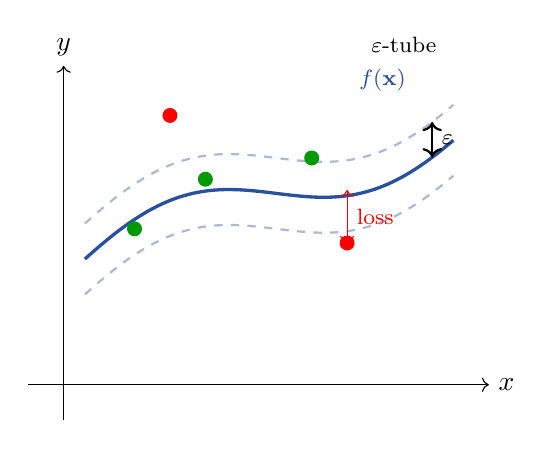
\begin{tikzpicture}[scale=0.9]
    \draw[->] (-0.5, 0) -- (6, 0) node[right] {$x$};
    \draw[->] (0, -0.5) -- (0, 4.5) node[above] {$y$};

    % Regression curve
    \draw[circuitblue, very thick, domain=0.3:5.5, smooth]
        plot (\x, {1.5 + 0.4*\x + 0.5*sin(\x*60)});

    % Epsilon tube
    \draw[circuitblue!40, thick, dashed, domain=0.3:5.5, smooth]
        plot (\x, {1.5 + 0.4*\x + 0.5*sin(\x*60) + 0.5});
    \draw[circuitblue!40, thick, dashed, domain=0.3:5.5, smooth]
        plot (\x, {1.5 + 0.4*\x + 0.5*sin(\x*60) - 0.5});

    % Points inside tube (no loss)
    \fill[green!60!black] (1, 2.2) circle (3pt);
    \fill[green!60!black] (2, 2.9) circle (3pt);
    \fill[green!60!black] (3.5, 3.2) circle (3pt);

    % Points outside tube (loss)
    \fill[red] (1.5, 3.8) circle (3pt);
    \fill[red] (4, 2.0) circle (3pt);
    \draw[red, <->] (4, 2.0) -- (4, 2.75) node[midway, right, font=\footnotesize] {loss};

    % Epsilon label
    \draw[<->, thick] (5.2, {1.5 + 0.4*5.2 + 0.5*sin(5.2*60)})
        -- (5.2, {1.5 + 0.4*5.2 + 0.5*sin(5.2*60) + 0.5});
    \node[right, font=\footnotesize] at (5.2, {1.5 + 0.4*5.2 + 0.5*sin(5.2*60) + 0.25}) {$\varepsilon$};

    \node[circuitblue, font=\footnotesize] at (4.5, 4.3) {$f(\mathbf{x})$};
    \node[font=\footnotesize] at (4.8, 4.8) {$\varepsilon$-tube};
\end{tikzpicture}
\end{center}

\subsection{QSVR Optimization}

\begin{definition}[QSVR Primal Problem]
\[
\min_{\mathbf{w}, b, \boldsymbol{\xi}, \boldsymbol{\xi}^*} \frac{1}{2}\|\mathbf{w}\|^2 + C \sum_{i=1}^M (\xi_i + \xi_i^*)
\]
subject to:
\begin{align}
y_i - \mathbf{w} \cdot \phi(\mathbf{x}_i) - b &\leq \varepsilon + \xi_i \\
\mathbf{w} \cdot \phi(\mathbf{x}_i) + b - y_i &\leq \varepsilon + \xi_i^* \\
\xi_i, \xi_i^* &\geq 0
\end{align}
\end{definition}

the dual problem introduces two sets of lagrange multipliers $\alpha_i$ and $\alpha_i^*$:

\begin{definition}[QSVR Dual Problem]
\[
\max_{\boldsymbol{\alpha}, \boldsymbol{\alpha}^*} -\frac{1}{2}\sum_{i,j=1}^M (\alpha_i - \alpha_i^*)(\alpha_j - \alpha_j^*) K_{ij} - \varepsilon \sum_{i=1}^M (\alpha_i + \alpha_i^*) + \sum_{i=1}^M y_i (\alpha_i - \alpha_i^*)
\]
subject to:
\begin{align}
\sum_{i=1}^M (\alpha_i - \alpha_i^*) &= 0 \\
0 \leq \alpha_i, \alpha_i^* &\leq C
\end{align}
\end{definition}

the regression function:
\[
f(\mathbf{x}) = \sum_{i=1}^M (\alpha_i^* - \alpha_i) \kappa(\mathbf{x}, \mathbf{x}_i) + b
\]

\begin{keypoint}
in QSVR, support vectors r points that lie \emph{on or outside} the $\varepsilon$-tube. points inside the tube have $\alpha_i = \alpha_i^* = 0$ and dont contribute to the regression function. the value of $\varepsilon$ controls how many support vectors u get: larger $\varepsilon$ = fewer support vectors = sparser model = faster prediction.
\end{keypoint}

\subsection{Choosing $\varepsilon$ and $C$}

\begin{itemize}[leftmargin=*]
    \item \textbf{$\varepsilon$}: controls the width of the tube. typical values: $0.01$ to $0.5$, depending on the noise level in ur data. rule of thumb: set $\varepsilon$ to be slightly larger than the expected noise standard deviation.

    \item \textbf{$C$}: regularization parameter. large $C$ = less regularization = fit the data more tightly (might overfit). small $C$ = more regularization = smoother function (might underfit).

    \item for quantum kernels, u typically want moderate $C$ (1 to 100) bcs the kernel itself provides implicit regularization through its structure.
\end{itemize}

%% ========================================================
\section{Pegasos QSVC}
%% ========================================================

standard SVM solvers (like libsvm used by sklearn) solve the dual problem exactly, which requires storing and manipulating the full $M \times M$ kernel matrix. for quantum kernels, this means computing all $O(M^2)$ kernel entries upfront.

the pegasos algorithm offers an alternative: stochastic gradient descent on the primal SVM objective, which only needs kernel evaluations for sampled data points at each step.

\subsection{The Pegasos Algorithm}

\begin{definition}[Pegasos (Primal Estimated sub-GrAdient SOlver for SVM)]
shalev-shwartz et al. (2011) proposed the following online algorithm:

initialize $\mathbf{w}_1 = \mathbf{0}$, step size $\eta_t = \frac{1}{\lambda t}$

for $t = 1, 2, \ldots, T$:
\begin{enumerate}[leftmargin=*]
    \item sample a mini-batch $A_t \subset \{1, \ldots, M\}$ of size $k$
    \item compute the subgradient:
    \[
    A_t^+ = \{i \in A_t : y_i (\mathbf{w}_t \cdot \phi(\mathbf{x}_i)) < 1\}
    \]
    \item update:
    \[
    \mathbf{w}_{t+1} = (1 - \eta_t \lambda) \mathbf{w}_t + \frac{\eta_t}{|A_t|} \sum_{i \in A_t^+} y_i \phi(\mathbf{x}_i)
    \]
    \item project: $\mathbf{w}_{t+1} = \min\!\left(1, \frac{1/\sqrt{\lambda}}{\|\mathbf{w}_{t+1}\|}\right) \mathbf{w}_{t+1}$
\end{enumerate}
\end{definition}

in kernel form, the weight vector is represented as:
\[
\mathbf{w}_t = \sum_{i=1}^M \beta_i^{(t)} \phi(\mathbf{x}_i)
\]

so the decision function $\mathbf{w}_t \cdot \phi(\mathbf{x}) = \sum_i \beta_i^{(t)} \kappa(\mathbf{x}_i, \mathbf{x})$ only requires kernel evaluations.

\subsection{Pegasos vs Standard SVM}

\begin{center}
\renewcommand{\arraystretch}{1.4}
\begin{tabular}{|l|c|c|}
\hline
\textbf{Property} & \textbf{Standard SVM (libsvm)} & \textbf{Pegasos} \\
\hline
kernel evaluations & $O(M^2)$ upfront & $O(kT)$ over training \\
\hline
memory & $O(M^2)$ for kernel matrix & $O(M)$ for coefficients \\
\hline
solution quality & exact (up to solver tol) & approximate \\
\hline
convergence & finite (QP solver) & $O(1/(\lambda \epsilon))$ iterations \\
\hline
mini-batch friendly & no & yes \\
\hline
\end{tabular}
\end{center}

\begin{keypoint}
the key advantage of pegasos for quantum kernels: u dont need to compute the full $M \times M$ kernel matrix. at each iteration, u only need kernel evaluations for the mini-batch. if the mini-batch size is $k$ and u do $T$ iterations, u need $O(kTM)$ kernel evaluations in the worst case (if all training points become part of the representation). in practice, its much less.
\end{keypoint}

\subsection{When to Use Pegasos QSVC}

\begin{itemize}[leftmargin=*]
    \item \textbf{larger datasets} ($M > 200$): the $O(M^2)$ cost of full kernel matrix becomes painful. pegasos lets u train with a ``budget'' of kernel evaluations.

    \item \textbf{online/streaming settings}: new data arrives over time. pegasos naturally handles this without recomputing the full kernel matrix.

    \item \textbf{when approximate is good enough}: pegasos converges to a solution thats close to optimal. for noisy quantum kernels, the kernel matrix itself is approximate, so an approximate solver is fine.

    \item \textbf{not recommended when}: $M$ is small ($< 100$), u need the exact SVM solution, or the kernel is cheap to compute (classical kernels).
\end{itemize}

\subsection{Convergence Analysis}

\begin{theorem}[Pegasos Convergence]
after $T$ iterations with mini-batch size $k = 1$, pegasos achieves:
\[
\mathbb{E}[f(\mathbf{w}_T)] - f(\mathbf{w}^*) \leq \frac{c}{\lambda T}
\]
where $f$ is the SVM objective, $\mathbf{w}^*$ is the optimal solution, and $c$ is a constant depending on the kernel bound $\max_i \kappa(\mathbf{x}_i, \mathbf{x}_i) \leq R^2$.

for quantum kernels, $\kappa(\mathbf{x}_i, \mathbf{x}_i) = 1$ always (fidelity of a state with itself), so $R^2 = 1$.
\end{theorem}

this means after $T = \frac{c}{\lambda \epsilon}$ iterations, we have $\epsilon$-optimal solution. with $\lambda = 1/C$:
\[
T = O\!\left(\frac{C}{\epsilon}\right)
\]

for $C = 10$ and $\epsilon = 0.01$, thats about $T = 1000$ iterations. with mini-batch size $k = 5$, thats $5000$ kernel evaluations --- much less than the $M^2/2$ needed for the full matrix when $M > 100$.

%% ========================================================
\section{Kernel Matrix Analysis}
%% ========================================================

understanding ur kernel matrix is crucial. the eigenvalue spectrum tells u a lot about whether the kernel is useful.

\subsection{Eigenvalue Decomposition}

the kernel matrix $K \in \mathbb{R}^{M \times M}$ is symmetric positive semi-definite (in the ideal case). its eigendecomposition is:
\[
K = \sum_{i=1}^M \lambda_i \mathbf{v}_i \mathbf{v}_i^\top, \quad \lambda_1 \geq \lambda_2 \geq \cdots \geq \lambda_M \geq 0
\]

\begin{definition}[Effective Rank]
the effective rank of the kernel matrix is:
\[
r_{\text{eff}}(K) = \exp\!\left(-\sum_{i=1}^M \frac{\lambda_i}{\text{tr}(K)} \log \frac{\lambda_i}{\text{tr}(K)}\right)
\]
this is the exponential of the entropy of the normalized eigenvalue distribution. it ranges from 1 (one dominant eigenvalue) to $M$ (all eigenvalues equal).
\end{definition}

\subsection{What the Spectrum Tells U}

\begin{center}
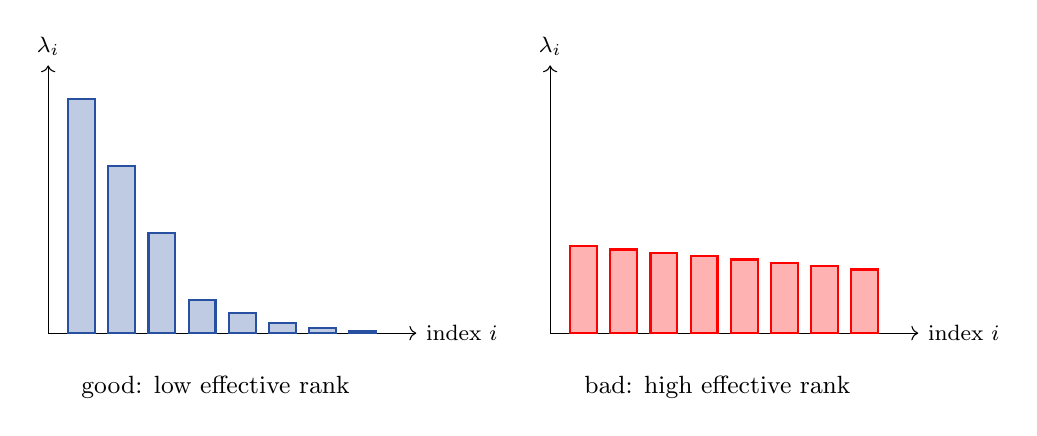
\begin{tikzpicture}[scale=0.85]
    % Good spectrum - few large eigenvalues
    \begin{scope}
        \draw[->] (0,0) -- (5.5,0) node[right, font=\footnotesize] {index $i$};
        \draw[->] (0,0) -- (0,4) node[above, font=\footnotesize] {$\lambda_i$};
        \draw[circuitblue, thick, fill=circuitblue!30]
            (0.3, 3.5) rectangle (0.7, 0)
            (0.9, 2.5) rectangle (1.3, 0)
            (1.5, 1.5) rectangle (1.9, 0)
            (2.1, 0.5) rectangle (2.5, 0)
            (2.7, 0.3) rectangle (3.1, 0)
            (3.3, 0.15) rectangle (3.7, 0)
            (3.9, 0.08) rectangle (4.3, 0)
            (4.5, 0.03) rectangle (4.9, 0);
        \node[below, font=\small] at (2.5, -0.5) {good: low effective rank};
    \end{scope}

    % Bad spectrum - all eigenvalues similar
    \begin{scope}[xshift=7.5cm]
        \draw[->] (0,0) -- (5.5,0) node[right, font=\footnotesize] {index $i$};
        \draw[->] (0,0) -- (0,4) node[above, font=\footnotesize] {$\lambda_i$};
        \draw[red, thick, fill=red!30]
            (0.3, 1.3) rectangle (0.7, 0)
            (0.9, 1.25) rectangle (1.3, 0)
            (1.5, 1.2) rectangle (1.9, 0)
            (2.1, 1.15) rectangle (2.5, 0)
            (2.7, 1.1) rectangle (3.1, 0)
            (3.3, 1.05) rectangle (3.7, 0)
            (3.9, 1.0) rectangle (4.3, 0)
            (4.5, 0.95) rectangle (4.9, 0);
        \node[below, font=\small] at (2.5, -0.5) {bad: high effective rank};
    \end{scope}
\end{tikzpicture}
\end{center}

interpretation of different eigenvalue patterns:

\begin{enumerate}[leftmargin=*]
    \item \textbf{few large eigenvalues, rapid decay} ($r_{\text{eff}} \ll M$): the kernel captures a few important directions. this is good --- the SVM will find a good classifier in a low-dimensional effective subspace.

    \item \textbf{all eigenvalues similar} ($r_{\text{eff}} \approx M$): the kernel is essentially random. every direction is equally (un)important. this means the kernel doesnt encode useful structure. this often happens when:
    \begin{itemize}[leftmargin=*]
        \item too many qubits (exponential concentration)
        \item feature map is not matched to the data structure
        \item too much noise in the kernel estimates
    \end{itemize}

    \item \textbf{one very large eigenvalue, rest small}: the kernel is almost constant --- all data points look similar. this means the feature map maps everything to roughly the same quantum state.

    \item \textbf{negative eigenvalues}: the estimated kernel matrix is not PSD. this happens due to finite shot noise. small negative eigenvalues ($|\lambda_{\min}| < 0.01$) r fine --- just clip them. large negative eigenvalues indicate a problem.
\end{enumerate}

\subsection{Connection to SVM Performance}

\begin{theorem}[Eigenvalue Spectrum and Generalization]
the generalization error of the SVM trained with kernel $K$ is related to the eigenvalue spectrum through:
\[
\text{expected error} \leq O\!\left(\frac{1}{M} \sum_{i=1}^M \min\!\left(\frac{1}{C \lambda_i}, 1\right)\right)
\]
this bound is tightest when a few eigenvalues r large (corresponding to the useful features) and the rest r small (noise directions that get regularized away).
\end{theorem}

\begin{intuition}
think of eigenvalues as ``feature importances'' in the quantum feature space. large eigenvalues correspond to directions where data points vary a lot --- these r the useful features. small eigenvalues correspond to noise directions. the SVM naturally focuses on the large-eigenvalue directions (bcs they have more signal), so a kernel with a few large eigenvalues is ideal.
\end{intuition}

%% ========================================================
\section{Training on Real Datasets}
%% ========================================================

now lets get serious and look at training quantum kernel SVMs on actual (well, standard ML benchmark) datasets.

\subsection{Iris Dataset}

\textbf{dataset}: 150 samples, 4 features, 3 classes (setosa, versicolor, virginica).

\textbf{preprocessing}:
\begin{enumerate}[leftmargin=*]
    \item select 2 classes for binary classification (versicolor vs virginica --- the harder pair)
    \item select 2 features (petal length and width --- the most discriminative)
    \item standard scaling then rescale to $[0, \pi]$
    \item 70/30 train/test split, stratified
\end{enumerate}

\textbf{quantum setup}: 2 qubits, ZZFeatureMap, reps=2, full entanglement, 1024 shots.

\textbf{approach}: compute the full kernel matrix for training data ($\sim 70 \times 70 / 2 \approx 2450$ circuits). train QSVC with $C = 1.0$. compute test kernel matrix ($\sim 30 \times 70 = 2100$ circuits). predict on test set.

\textbf{expected results}:
\begin{itemize}[leftmargin=*]
    \item training accuracy: $\sim 93$--$96\%$
    \item test accuracy: $\sim 90$--$95\%$
    \item number of support vectors: $\sim 15$--$25$
    \item kernel alignment: $\sim 0.15$--$0.25$
\end{itemize}

\textbf{comparison}: classical RBF kernel with tuned $\gamma$ typically gets $95$--$97\%$ test accuracy. so quantum is close but slightly below.

\subsection{Wine Dataset}

\textbf{dataset}: 178 samples, 13 features, 3 classes.

\textbf{preprocessing}: this is where it gets tricky --- 13 features but we can only use $n$ qubits.
\begin{enumerate}[leftmargin=*]
    \item select 2 classes (class 1 vs class 2)
    \item apply PCA to reduce to 4 features (4 qubits)
    \item standard scaling then rescale to $[0, \pi]$
    \item 70/30 train/test split
\end{enumerate}

\textbf{quantum setup}: 4 qubits, ZZFeatureMap, reps=2, linear entanglement, 2048 shots.

\textbf{why linear entanglement}: with 4 qubits, full entanglement gives $\binom{4}{2} = 6$ ZZ interactions per layer. the circuit depth becomes $\sim 40$ gates per rep, so the kernel circuit has $\sim 160$ gates. with linear entanglement (3 ZZ interactions per layer), depth drops to $\sim 100$ gates. on noisy hardware, this matters a lot.

\textbf{expected results}:
\begin{itemize}[leftmargin=*]
    \item training accuracy: $\sim 90$--$95\%$
    \item test accuracy: $\sim 85$--$92\%$
    \item kernel alignment: $\sim 0.10$--$0.20$
\end{itemize}

\begin{intuition}
the wine dataset is harder for quantum kernels bcs the PCA step throws away information that might be in the discarded principal components. classical kernels operating on all 13 features have an inherent advantage here. this illustrates a fundamental limitation: quantum kernels r constrained by the number of available qubits.
\end{intuition}

\subsection{Breast Cancer Dataset}

\textbf{dataset}: 569 samples, 30 features, 2 classes (malignant vs benign).

\textbf{preprocessing}:
\begin{enumerate}[leftmargin=*]
    \item PCA to 4 features (explaining $\sim 95\%$ of variance)
    \item standard scaling then rescale to $[0, \pi]$
    \item 70/30 train/test split, stratified
\end{enumerate}

\textbf{quantum setup}: 4 qubits, ZZFeatureMap, reps=2, 2048 shots.

\textbf{expected results}:
\begin{itemize}[leftmargin=*]
    \item training accuracy: $\sim 92$--$96\%$
    \item test accuracy: $\sim 90$--$95\%$
    \item kernel alignment: $\sim 0.20$--$0.30$
\end{itemize}

\textbf{computational cost}: $M_{\text{train}} \approx 400$, so we need $\sim 80{,}000$ circuits for the training kernel matrix. at 2048 shots each, thats $\sim 164$ million circuit shots. on a simulator, this takes minutes. on real hardware, this is a significant job.

\begin{keypoint}
with 569 samples, the breast cancer dataset pushes the limits of quantum kernel methods. the $O(M^2)$ scaling means $\sim 160{,}000$ kernel evaluations. this is where pegasos QSVC becomes attractive --- it can train with a fraction of the kernel evaluations.
\end{keypoint}

%% ========================================================
\section{Cross-Validation with Quantum Kernels}
%% ========================================================

cross-validation is essential for honest performance evaluation, but its expensive with quantum kernels.

\subsection{The Cost Problem}

for $k$-fold cross-validation:
\begin{itemize}[leftmargin=*]
    \item $k$ different train/test splits
    \item each split requires a new kernel matrix (different training set $\to$ different kernel entries needed)
    \item naive approach: $k$ full kernel matrix computations
\end{itemize}

total cost without optimization:
\[
\text{cost}_{\text{naive}} = k \cdot \frac{M_{\text{train}}(M_{\text{train}} - 1)}{2} \cdot N_s
\]

for $k = 5$, $M = 100$, $N_s = 1024$: thats $5 \times 4950 \times 1024 \approx 25$ million circuit shots.

\subsection{Smart Cross-Validation}

\begin{keypoint}
the key insight: compute the full $M \times M$ kernel matrix \emph{once} using all data points. then for each fold, extract the relevant submatrix. this works bcs $\kappa(\mathbf{x}_i, \mathbf{x}_j)$ doesnt depend on which fold ur in --- the kernel value between two points is always the same.
\end{keypoint}

the procedure:
\begin{enumerate}[leftmargin=*]
    \item compute the full kernel matrix $K \in \mathbb{R}^{M \times M}$ --- cost: $\frac{M(M-1)}{2} \cdot N_s$
    \item for each fold $f = 1, \ldots, k$:
    \begin{itemize}[leftmargin=*]
        \item let $\mathcal{I}_f^{\text{train}}$ and $\mathcal{I}_f^{\text{test}}$ be the train and test indices
        \item extract $K_{\text{train}}^{(f)} = K[\mathcal{I}_f^{\text{train}}, \mathcal{I}_f^{\text{train}}]$
        \item extract $K_{\text{test}}^{(f)} = K[\mathcal{I}_f^{\text{test}}, \mathcal{I}_f^{\text{train}}]$
        \item train SVM with $K_{\text{train}}^{(f)}$ (this is fast --- classical computation)
        \item predict using $K_{\text{test}}^{(f)}$
    \end{itemize}
    \item average the scores across folds
\end{enumerate}

total cost:
\[
\text{cost}_{\text{smart}} = \frac{M(M-1)}{2} \cdot N_s + k \cdot \text{(classical SVM cost)}
\]

the classical SVM cost is negligible compared to the quantum kernel computation. so smart cross-validation is essentially free once u have the full kernel matrix.

\subsection{Nested Cross-Validation}

for honest hyperparameter tuning, u need nested cross-validation: an outer loop for performance estimation and an inner loop for hyperparameter selection.

the problem: if u change the feature map hyperparameters (reps, entanglement), u need a \emph{new} kernel matrix. so for $p$ hyperparameter settings, u need $p$ full kernel matrices.

\begin{align}
\text{cost}_{\text{nested}} &= p \cdot \frac{M(M-1)}{2} \cdot N_s \\
&+ k_{\text{outer}} \cdot k_{\text{inner}} \cdot \text{(classical SVM cost)}
\end{align}

for $p = 10$ hyperparameter settings, $M = 100$, $N_s = 1024$: thats $10 \times 4950 \times 1024 \approx 50$ million circuit shots. still feasible on a simulator, but getting expensive on real hardware.

%% ========================================================
\section{Hyperparameter Tuning}
%% ========================================================

quantum kernel SVMs have several hyperparameters to tune. lets go through them systematically.

\subsection{Feature Map Parameters}

\begin{enumerate}[leftmargin=*]
    \item \textbf{feature map type}: ZFeatureMap, ZZFeatureMap, PauliFeatureMap, or custom. start with ZZFeatureMap --- its the standard choice with a good expressivity/cost tradeoff.

    \item \textbf{number of repetitions (reps)}: controls depth and expressivity.
    \begin{itemize}[leftmargin=*]
        \item reps=1: shallow, less expressive, more noise-robust
        \item reps=2: good default, reasonable depth
        \item reps=3+: deep, more expressive, noise-sensitive
    \end{itemize}
    recommendation: try reps $\in \{1, 2, 3\}$ and pick the best by cross-validation.

    \item \textbf{entanglement scheme}: full, linear, circular, or sca.
    \begin{itemize}[leftmargin=*]
        \item for $n \leq 4$ qubits: full is fine
        \item for $n \geq 5$ qubits: linear or circular to keep depth manageable
    \end{itemize}

    \item \textbf{data encoding function}: the default is $\phi_S(\mathbf{x}) = \prod_{j \in S} x_j$. alternatives include $\phi_S(\mathbf{x}) = \prod_{j \in S} (\pi - x_j)$ or polynomial functions of $x_j$.
\end{enumerate}

\subsection{SVM Hyperparameters}

\begin{enumerate}[leftmargin=*]
    \item \textbf{$C$ (regularization)}: the penalty for margin violations.
    \begin{itemize}[leftmargin=*]
        \item small $C$ ($0.01$--$0.1$): heavy regularization, smoother boundary, fewer support vectors
        \item moderate $C$ ($1$--$10$): balanced
        \item large $C$ ($100$+): little regularization, complex boundary, many support vectors
    \end{itemize}
    typical grid: $C \in \{0.1, 1, 10, 100\}$.

    \item \textbf{$\varepsilon$ (for QSVR)}: tube width.
    typical grid: $\varepsilon \in \{0.01, 0.05, 0.1, 0.2, 0.5\}$.
\end{enumerate}

\subsection{Tuning Strategy}

\begin{keypoint}
the most efficient tuning strategy for quantum kernels:
\begin{enumerate}[leftmargin=*]
    \item first, use kernel alignment (cheap to compute) to narrow down feature map choices. compute alignment for each candidate feature map and discard those with alignment $< 0.05$.
    \item then, for the surviving feature maps, do cross-validation to tune $C$ (and $\varepsilon$ for regression).
    \item finally, evaluate the best configuration on a held-out test set.
\end{enumerate}
this saves a lot of quantum computation bcs alignment doesnt require SVM training.
\end{keypoint}

the quantikz circuits for comparing different feature maps:

\textbf{ZFeatureMap (no entanglement):}
\begin{center}
\begin{quantikz}
    \lstick{$\ket{0}$} & \gate{H} & \gate{R_Z(x_1)} & \gate{H} & \gate{R_Z(x_1)} & \qw \\
    \lstick{$\ket{0}$} & \gate{H} & \gate{R_Z(x_2)} & \gate{H} & \gate{R_Z(x_2)} & \qw
\end{quantikz}
\end{center}

\textbf{ZZFeatureMap (pairwise entanglement):}
\begin{center}
\begin{quantikz}
    \lstick{$\ket{0}$} & \gate{H} & \gate{R_Z(x_1)} & \ctrl{1} & \qw & \gate{H} & \gate{R_Z(x_1)} & \ctrl{1} & \qw \\
    \lstick{$\ket{0}$} & \gate{H} & \gate{R_Z(x_2)} & \gate{R_Z(x_1 x_2)} & \qw & \gate{H} & \gate{R_Z(x_2)} & \gate{R_Z(x_1 x_2)} & \qw
\end{quantikz}
\end{center}

\textbf{PauliFeatureMap with Y and ZZ:}
\begin{center}
\begin{quantikz}
    \lstick{$\ket{0}$} & \gate{H} & \gate{R_Y(x_1)} & \ctrl{1} & \qw & \gate{H} & \gate{R_Y(x_1)} & \ctrl{1} & \qw \\
    \lstick{$\ket{0}$} & \gate{H} & \gate{R_Y(x_2)} & \gate{R_Z(x_1 x_2)} & \qw & \gate{H} & \gate{R_Y(x_2)} & \gate{R_Z(x_1 x_2)} & \qw
\end{quantikz}
\end{center}

note how the ZFeatureMap has no two-qubit gates, while ZZFeatureMap and PauliFeatureMap include controlled rotations that create entanglement dependent on the data.

%% ========================================================
\section{Computational Cost Analysis}
%% ========================================================

lets be rigorous about the computational costs. this is important bcs quantum kernels r often presented as ``working'' without mentioning how expensive they r.

\subsection{Kernel Matrix Construction}

\begin{definition}[Quantum Kernel Computation Cost]
for $M$ data points, $n$ qubits, feature map depth $D$ (in gates), and $N_s$ shots:
\begin{align}
\text{unique circuits} &= \frac{M(M-1)}{2} \\
\text{gates per circuit} &= 2D \quad \text{(compute-uncompute)} \\
\text{total shots} &= \frac{M(M-1)}{2} \cdot N_s \\
\text{total gate operations} &= \frac{M(M-1)}{2} \cdot N_s \cdot 2D
\end{align}
\end{definition}

lets put real numbers on this:

\begin{center}
\renewcommand{\arraystretch}{1.3}
\begin{tabular}{|c|c|c|c|c|}
\hline
$M$ & $N_s$ & circuits & total shots & time (sim) \\
\hline
50 & 1024 & 1,225 & 1.25M & $\sim 10$s \\
\hline
100 & 1024 & 4,950 & 5.07M & $\sim 1$min \\
\hline
200 & 1024 & 19,900 & 20.4M & $\sim 5$min \\
\hline
500 & 1024 & 124,750 & 127.7M & $\sim 30$min \\
\hline
1000 & 1024 & 499,500 & 511.5M & $\sim 2$hrs \\
\hline
\end{tabular}
\end{center}

(times r rough estimates for a statevector simulator on a modern laptop. actual hardware times depend on queue and calibration.)

\subsection{Prediction Cost}

for a new test point, u need $|\mathcal{SV}|$ kernel evaluations (one per support vector). each requires $N_s$ shots.

\[
\text{prediction cost per point} = |\mathcal{SV}| \cdot N_s \cdot 2D \text{ gate operations}
\]

if the SVM has 30 support vectors and $N_s = 1024$: thats 30,720 circuit shots per prediction. not terrible, but not instant either.

\subsection{Comparison with Classical Kernels}

\begin{center}
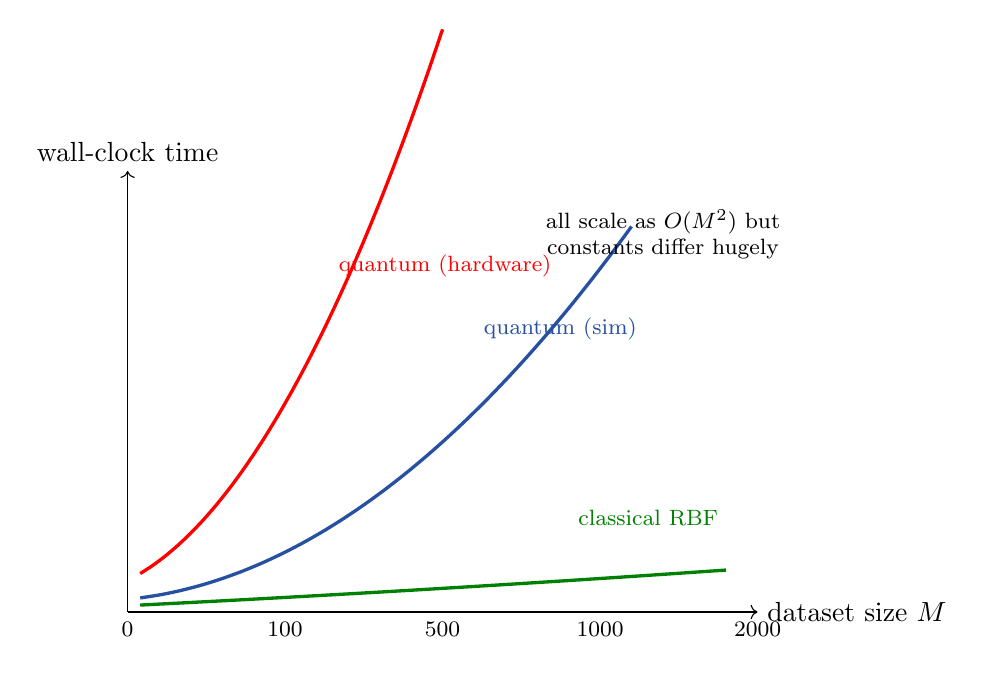
\begin{tikzpicture}[scale=0.8]
    \draw[->] (0,0) -- (10,0) node[right] {dataset size $M$};
    \draw[->] (0,0) -- (0,7) node[above] {wall-clock time};

    % Axis labels
    \node[below, font=\footnotesize] at (0,0) {0};
    \node[below, font=\footnotesize] at (2.5,0) {100};
    \node[below, font=\footnotesize] at (5,0) {500};
    \node[below, font=\footnotesize] at (7.5,0) {1000};
    \node[below, font=\footnotesize] at (10,0) {2000};

    % Classical RBF
    \draw[green!50!black, very thick, domain=0.2:9.5, smooth]
        plot (\x, {0.001*\x*\x + 0.05*\x + 0.1});
    \node[green!50!black, right, font=\footnotesize] at (7, 1.5) {classical RBF};

    % Quantum kernel (simulator)
    \draw[circuitblue, very thick, domain=0.2:8, smooth]
        plot (\x, {0.08*\x*\x + 0.1*\x + 0.2});
    \node[circuitblue, right, font=\footnotesize] at (5.5, 4.5) {quantum (sim)};

    % Quantum kernel (hardware)
    \draw[red, very thick, domain=0.2:5, smooth]
        plot (\x, {0.25*\x*\x + 0.5*\x + 0.5});
    \node[red, right, font=\footnotesize] at (3.2, 5.5) {quantum (hardware)};

    % Note
    \node[font=\footnotesize, text width=3cm, align=center] at (8.5, 6) {all scale as $O(M^2)$ but constants differ hugely};
\end{tikzpicture}
\end{center}

the key point: quantum and classical kernels both scale as $O(M^2)$ for training, but the constant factor is \emph{enormously} different. computing $\kappa_{\text{RBF}}(\mathbf{x}, \mathbf{x}') = e^{-\gamma\|\mathbf{x} - \mathbf{x}'\|^2}$ takes nanoseconds. computing $\kappa_{\text{quantum}}(\mathbf{x}, \mathbf{x}')$ takes microseconds (simulator) to milliseconds (hardware per shot). thats a factor of $10^3$ to $10^6$.

\begin{keypoint}
quantum kernels can only justify their computational cost if they provide a classification/regression quality that classical kernels \emph{cannot match}, not just one that they \emph{happen not to match} with default hyperparameters. this is a very high bar.
\end{keypoint}

\subsection{Total Budget Planning}

for a practical quantum kernel experiment, plan ur compute budget:

\begin{align}
\text{total budget} &= \underbrace{p \cdot \frac{M(M-1)}{2} \cdot N_s}_{\text{hyperparameter search}} + \underbrace{\frac{M(M-1)}{2} \cdot N_s}_{\text{final training}} + \underbrace{M_{\text{test}} \cdot |\mathcal{SV}| \cdot N_s}_{\text{prediction}}
\end{align}

where $p$ is the number of hyperparameter configurations to try. for $p = 12$ (3 reps $\times$ 4 $C$ values), $M = 100$, $N_s = 1024$:
\[
\text{budget} = 12 \times 4950 \times 1024 + 4950 \times 1024 + 30 \times 20 \times 1024 \approx 66 \text{ million shots}
\]

%% ========================================================
\section{Classical vs Quantum Kernel Comparison}
%% ========================================================

when does quantum actually win? lets be precise.

\subsection{When Quantum Kernels Can Win}

\begin{theorem}[Quantum Advantage for Kernels (Liu, Arunachalam, Temme 2021)]
there exist classification problems where:
\begin{enumerate}[leftmargin=*]
    \item a quantum kernel achieves low prediction error
    \item any classical kernel (with polynomial-time computable entries) achieves high prediction error
\end{enumerate}
the separation is based on the hardness of the discrete logarithm problem and requires data with specific structure related to quantum computation.
\end{theorem}

\begin{intuition}
the proven quantum advantage is for \emph{constructed} problems where the data is specifically designed to be easy for quantum kernels. these r not natural ML problems --- theyre cryptographic in nature. for natural datasets, no proven advantage exists (yet).
\end{intuition}

\subsection{Empirical Comparison: Feature Map Expressivity}

on standard ML benchmarks, here is the typical picture:

\begin{center}
\renewcommand{\arraystretch}{1.4}
\begin{tabular}{|l|c|c|c|c|}
\hline
\textbf{Kernel} & \textbf{Iris} & \textbf{Wine} & \textbf{Cancer} & \textbf{Compute} \\
\hline
linear & $87\%$ & $95\%$ & $95\%$ & fast \\
\hline
RBF (tuned) & $95\%$ & $98\%$ & $97\%$ & fast \\
\hline
polynomial (tuned) & $93\%$ & $97\%$ & $96\%$ & fast \\
\hline
quantum ZFeatureMap & $88\%$ & $90\%$ & $92\%$ & slow \\
\hline
quantum ZZFeatureMap & $93\%$ & $93\%$ & $94\%$ & slow \\
\hline
quantum PauliFeatureMap & $94\%$ & $94\%$ & $95\%$ & very slow \\
\hline
\end{tabular}
\end{center}

\begin{keypoint}
on standard benchmark datasets, quantum kernels perform comparably to classical kernels but r orders of magnitude slower. the quantum kernels with entanglement (ZZFeatureMap, PauliFeatureMap) consistently outperform those without (ZFeatureMap), confirming that entanglement adds expressivity. but classical RBF with tuned $\gamma$ is very hard to beat.
\end{keypoint}

\subsection{When Quantum Doesnt Win}

be honest about the limitations:

\begin{enumerate}[leftmargin=*]
    \item \textbf{smooth low-dimensional data}: if the decision boundary is smooth and the data lives in low dimensions, RBF kernel captures it perfectly. quantum kernels cant do better bcs theres nothing more to capture.

    \item \textbf{high-dimensional data with linear structure}: if the data is linearly separable in the original space (or after a simple feature engineering step), a linear kernel suffices. adding quantum complexity is wasteful.

    \item \textbf{very noisy data}: if the bayes-optimal error is high (say $> 20\%$), no kernel (quantum or classical) will do well. the noise floor is a fundamental limit.

    \item \textbf{large datasets}: the $O(M^2)$ cost makes quantum kernels impractical for $M > 1000$ on current hardware.
\end{enumerate}

%% ========================================================
\section{Limitations and When NOT to Use Quantum Kernels}
%% ========================================================

this section is arguably the most important in the whole lecture. knowing when \emph{not} to use a method is just as valuable as knowing when to use it.

\subsection{Dataset Size Limits}

the $O(M^2)$ kernel matrix is the fundamental bottleneck:

\begin{center}
\renewcommand{\arraystretch}{1.3}
\begin{tabular}{|c|c|c|l|}
\hline
$M$ & kernel entries & at 1024 shots & \textbf{feasibility} \\
\hline
50 & 1,225 & 1.25M shots & easy \\
\hline
100 & 4,950 & 5.07M shots & comfortable \\
\hline
500 & 124,750 & 127.7M shots & challenging \\
\hline
1,000 & 499,500 & 511.5M shots & hard \\
\hline
10,000 & 49,995,000 & 51.2B shots & impossible (current hw) \\
\hline
\end{tabular}
\end{center}

\begin{keypoint}
practical limit with current quantum hardware: $M \leq 200$--$500$ depending on the number of qubits and shots. with simulators, u can push to $M \sim 1000$, but the classical simulation itself becomes slow for $n > 20$ qubits.
\end{keypoint}

\subsection{Noise Sensitivity}

recall from last lecture: noise pushes all kernel values toward $1/2^n$. the signal-to-noise ratio of the kernel:

\[
\text{SNR} = \frac{|\kappa_{\text{ideal}}(\mathbf{x}, \mathbf{x}') - 1/2^n|}{1/\sqrt{N_s}} \cdot (1-p)^{2D_{\text{gates}}}
\]

for the kernel to be useful, u need $\text{SNR} \gg 1$. this constrains:
\begin{itemize}[leftmargin=*]
    \item number of qubits $n$ (bcs of $1/2^n$ noise floor)
    \item circuit depth $D_{\text{gates}}$ (bcs of exponential fidelity decay)
    \item number of shots $N_s$ (bcs of statistical noise)
\end{itemize}

\subsection{The Concentration Problem}

\begin{definition}[Kernel Concentration]
a kernel $\kappa$ exhibits concentration if for random data points $\mathbf{x}, \mathbf{x}'$:
\[
\text{Var}_{\mathbf{x}, \mathbf{x}'}[\kappa(\mathbf{x}, \mathbf{x}')] \to 0 \text{ as } n \to \infty
\]
meaning all off-diagonal kernel entries converge to the same value. the kernel becomes uninformative.
\end{definition}

\begin{theorem}[Exponential Concentration (Thanasilp et al., 2022)]
for the standard quantum kernel with $n$ qubits and feature maps forming approximate 2-designs:
\[
\text{Var}_{\mathbf{x}, \mathbf{x}'}[\kappa(\mathbf{x}, \mathbf{x}')] \leq O\!\left(\frac{1}{2^n}\right)
\]
the kernel concentrates exponentially in the number of qubits.
\end{theorem}

\begin{intuition}
this is the quantum kernel version of the ``curse of dimensionality.'' as u add more qubits, the hilbert space grows as $2^n$, and random quantum states become nearly orthogonal. the kernel value between any two random points approaches $1/2^n \approx 0$, and the variance around this value shrinks exponentially. the kernel matrix becomes $K \approx I$ (identity), which is useless for classification.
\end{intuition}

ways to mitigate concentration:
\begin{enumerate}[leftmargin=*]
    \item use fewer qubits (match to the intrinsic dimensionality of the data)
    \item use projected quantum kernels (measure local observables instead of global fidelity)
    \item use shallow circuits with limited entanglement
    \item use data-dependent feature maps trained to avoid concentration
\end{enumerate}

\subsection{When NOT to Use Quantum Kernels}

a definitive list:

\begin{enumerate}[leftmargin=*]
    \item \textbf{dataset has $> 1000$ samples}: the $O(M^2)$ cost is prohibitive. use a classical kernel SVM, random features approximation, or a neural network instead.

    \item \textbf{data is high-dimensional and u need many qubits}: if $n > 10$ qubits, concentration will likely kill performance. either reduce dimensionality aggressively or use a different approach.

    \item \textbf{classical RBF kernel already works well}: if u can get $> 95\%$ accuracy with a tuned RBF kernel, adding quantum complexity wont help (and will cost orders of magnitude more compute).

    \item \textbf{running on very noisy hardware}: if gate error rates r above $1\%$ and ur circuit has $> 50$ gates, the kernel signal will be drowned in noise.

    \item \textbf{real-time prediction is needed}: each prediction requires $|\mathcal{SV}|$ quantum circuit evaluations. this is too slow for real-time applications.

    \item \textbf{interpretability is important}: quantum kernels r black boxes on top of black boxes. if u need to explain why the model makes a decision, use a simpler model.
\end{enumerate}

\subsection{Decision Flowchart}

\begin{center}
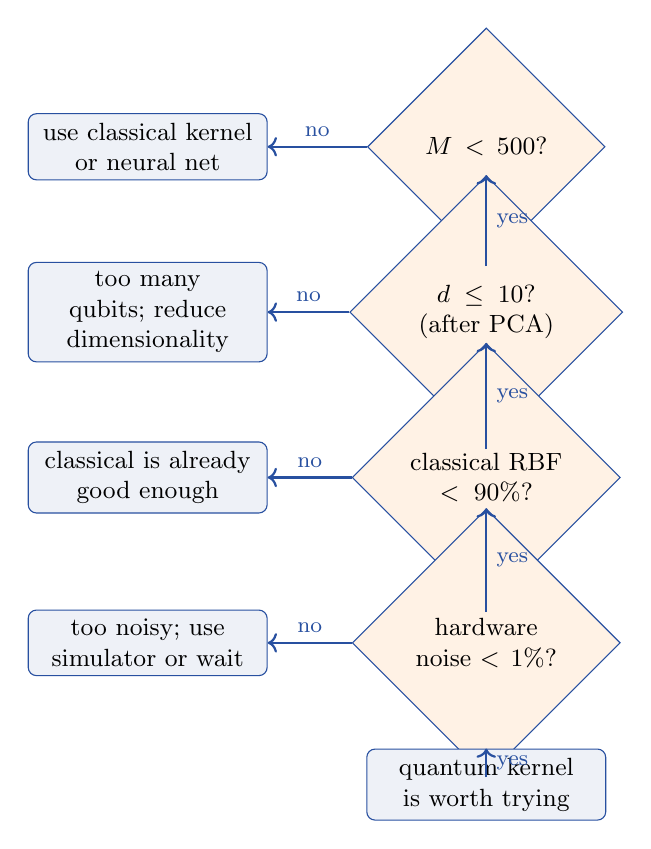
\begin{tikzpicture}[
    node distance=1.3cm,
    decision/.style={diamond, draw=circuitblue, fill=orange!10,
        text width=2.5cm, align=center, font=\small, inner sep=2pt},
    result/.style={rectangle, draw=circuitblue, fill=circuitblue!8,
        minimum width=2.5cm, minimum height=0.7cm, rounded corners=3pt,
        font=\small, text width=2.8cm, align=center},
    arrow/.style={->, thick, circuitblue}
]
    \node[decision] (q1) {$M < 500$?};
    \node[result, left of=q1, xshift=-3cm] (r1) {use classical kernel or neural net};
    \node[decision, below of=q1, yshift=-0.8cm] (q2) {$d \leq 10$? (after PCA)};
    \node[result, left of=q2, xshift=-3cm] (r2) {too many qubits; reduce dimensionality};
    \node[decision, below of=q2, yshift=-0.8cm] (q3) {classical RBF $< 90\%$?};
    \node[result, left of=q3, xshift=-3cm] (r3) {classical is already good enough};
    \node[decision, below of=q3, yshift=-0.8cm] (q4) {hardware noise $< 1\%$?};
    \node[result, left of=q4, xshift=-3cm] (r4) {too noisy; use simulator or wait};
    \node[result, below of=q4, yshift=-0.5cm] (r5) {quantum kernel is worth trying};

    \draw[arrow] (q1) -- node[above, font=\footnotesize] {no} (r1);
    \draw[arrow] (q1) -- node[right, font=\footnotesize] {yes} (q2);
    \draw[arrow] (q2) -- node[above, font=\footnotesize] {no} (r2);
    \draw[arrow] (q2) -- node[right, font=\footnotesize] {yes} (q3);
    \draw[arrow] (q3) -- node[above, font=\footnotesize] {no} (r3);
    \draw[arrow] (q3) -- node[right, font=\footnotesize] {yes} (q4);
    \draw[arrow] (q4) -- node[above, font=\footnotesize] {no} (r4);
    \draw[arrow] (q4) -- node[right, font=\footnotesize] {yes} (r5);
\end{tikzpicture}
\end{center}

%% ========================================================
\section{Advanced Topics}
%% ========================================================

\subsection{Trainable Quantum Kernels}

instead of using a fixed feature map, u can add trainable parameters:
\[
U(\mathbf{x}; \boldsymbol{\theta}) = V(\boldsymbol{\theta}) W(\mathbf{x}) V'(\boldsymbol{\theta})
\]

where $V(\boldsymbol{\theta})$ and $V'(\boldsymbol{\theta})$ r trainable unitaries and $W(\mathbf{x})$ is the data encoding. the parameters $\boldsymbol{\theta}$ r optimized to maximize kernel alignment:

\[
\boldsymbol{\theta}^* = \arg\max_{\boldsymbol{\theta}} A(K(\boldsymbol{\theta}), \mathbf{y}\mathbf{y}^\top)
\]

this is a quantum-classical optimization loop:
\begin{enumerate}[leftmargin=*]
    \item initialize $\boldsymbol{\theta}$ randomly
    \item compute kernel matrix $K(\boldsymbol{\theta})$
    \item compute alignment $A$ and its gradient w.r.t. $\boldsymbol{\theta}$
    \item update $\boldsymbol{\theta}$ using gradient ascent
    \item repeat until convergence
\end{enumerate}

the gradient of each kernel entry w.r.t. $\theta_k$ can be computed using the parameter shift rule:
\[
\frac{\partial K_{ij}}{\partial \theta_k} = \frac{K_{ij}(\theta_k + \pi/2) - K_{ij}(\theta_k - \pi/2)}{2}
\]

this requires computing two additional kernel matrices per parameter per gradient step. expensive, but can significantly improve kernel quality.

\subsection{Quantum Kernel Bandwidth}

by analogy with the RBF kernel ($k(\mathbf{x}, \mathbf{x}') = e^{-\gamma\|\mathbf{x} - \mathbf{x}'\|^2}$), quantum kernels have an implicit ``bandwidth'' controlled by the feature map scaling.

if u encode data as $U(\alpha \mathbf{x})$ where $\alpha$ is a scaling parameter:
\begin{itemize}[leftmargin=*]
    \item small $\alpha$: all quantum states r similar $\to$ kernel values close to 1 $\to$ underfitting
    \item large $\alpha$: all quantum states r different $\to$ kernel values close to 0 $\to$ overfitting
    \item optimal $\alpha$: depends on the data distribution
\end{itemize}

\begin{keypoint}
the data rescaling factor $\alpha$ acts like an inverse bandwidth for quantum kernels. tuning it is at least as important as tuning the feature map architecture. a good starting point is $\alpha = 1$ (data in $[0, \pi]$), then search over $\alpha \in \{0.5, 1, 2, 4\}$.
\end{keypoint}

\subsection{Kernel Principal Component Analysis}

u can use the quantum kernel matrix for dimensionality reduction via kernel PCA:

\begin{enumerate}[leftmargin=*]
    \item compute the $M \times M$ quantum kernel matrix $K$
    \item center the kernel: $\tilde{K} = K - \frac{1}{M}\mathbf{1}\mathbf{1}^\top K - K \frac{1}{M}\mathbf{1}\mathbf{1}^\top + \frac{1}{M^2}\mathbf{1}\mathbf{1}^\top K \mathbf{1}\mathbf{1}^\top$
    \item eigendecompose: $\tilde{K} = V \Lambda V^\top$
    \item project: new features r the columns of $V \Lambda^{1/2}$ (top $k$ components)
\end{enumerate}

the quantum kernel PCA features can then be used with \emph{any} classical ML algorithm, not just SVMs. this is a nice way to extract value from quantum kernels without committing to the SVM framework.

%% ========================================================
\section{Putting It All Together}
%% ========================================================

heres the recommended workflow for a quantum kernel project:

\begin{enumerate}[leftmargin=*]
    \item \textbf{baseline first}: train a classical SVM with RBF kernel, tune $\gamma$ and $C$. this is ur target to beat.

    \item \textbf{feasibility check}: is $M < 500$? is $d$ (after PCA) $\leq 10$? if no, dont bother with quantum kernels.

    \item \textbf{feature map selection}: compute kernel alignment for several feature maps (ZZFeatureMap with reps=1,2,3 and different entanglements). pick the top 2-3 by alignment.

    \item \textbf{cross-validation}: for each selected feature map, compute the full kernel matrix and do 5-fold CV over $C \in \{0.1, 1, 10, 100\}$.

    \item \textbf{compare}: is the best quantum kernel within $\pm 2\%$ of the classical baseline? if not, the classical kernel is better. if yes, report that quantum is ``competitive'' (not ``better'').

    \item \textbf{analyze}: look at the kernel matrix structure, eigenvalue spectrum, number of support vectors. understand \emph{why} the kernel works or doesnt.

    \item \textbf{report honestly}: include computational cost, noise analysis (if on real hardware), and comparison with classical baselines. dont cherry-pick.
\end{enumerate}

%% ========================================================
\section{Summary and Key Takeaways}
%% ========================================================

this lecture covered the practical and theoretical aspects of using quantum kernels with SVMs. the main points:

\begin{enumerate}[leftmargin=*]
    \item \textbf{QSVC and QSVR} r straightforward: plug a quantum kernel into a classical SVM. the math is identical to classical kernel SVMs --- the only difference is how the kernel entries r computed.

    \item \textbf{pegasos QSVC} offers a way to train without the full $O(M^2)$ kernel matrix. useful for larger datasets ($M > 200$) where computing all kernel entries is expensive.

    \item \textbf{eigenvalue analysis} of the kernel matrix tells u whether the kernel is informative. look for rapid eigenvalue decay (low effective rank) --- thats the sign of a useful kernel.

    \item \textbf{cross-validation is essential} but can be done efficiently by computing the full kernel matrix once and extracting submatrices for each fold.

    \item \textbf{hyperparameter tuning}: use alignment-based prefiltering, then cross-validation for $C$ (and $\varepsilon$). dont forget the data scaling factor $\alpha$.

    \item \textbf{computational cost is the elephant in the room}: quantum kernels r $10^3$--$10^6$ times slower per kernel entry than classical kernels. this cost is only justified if the quantum kernel provides genuinely better classification.

    \item \textbf{on standard benchmarks, classical wins or ties}: this is the honest conclusion from current research. quantum advantage for kernels has been \emph{proven to exist} for constructed problems, but not demonstrated for natural ML problems.

    \item \textbf{know when NOT to use quantum kernels}: large datasets, high-dimensional data, noisy hardware, or when classical already works well. this is perhaps the most important lesson.

    \item \textbf{the concentration problem} is fundamental: more qubits $\neq$ better kernels. match the number of qubits to the intrinsic dimensionality of ur data.

    \item \textbf{honest benchmarking}: always compare against tuned classical baselines, report computational costs, use proper cross-validation, and dont cherry-pick results.
\end{enumerate}

next lecture well move beyond kernels entirely and look at quantum neural networks and variational classifiers --- a completely different approach to quantum machine learning.

\end{document}
